\section{Review and Retrospective}

Generally the retrospective meetings were finished very quickly.

The team worked quite well and did not face any major issues during the sprints.

The main issues found were the work estimates, where some tasks took longer or less time than expected and some team members allocated either too much or too little to themselves.

Focusing on the documentation in the first sprint gave the team a solid foundation for the ensuing programming sprints, which was a great benefit.

Using \textit{SCRUM} proved to be very effective in planning the work. Having shorter sprints helped keep spirits up for team members, and ensured that everyone did not drown in work. The team was always able to see the end of the next sprint and how much work was left.

Using an iterative approach was a benefit and the team appreciated the ability to change course during the project.

Having a waterfall-like approach would not have given the team the same abilities to do this, and unexpected problems that were discovered during the project might not have been as easy to fix.

The fact that the team was relatively small and therefore well-suited for the \textit{SCRUM} methodology helped a great deal as well. Had the team been larger other issues might have surfaced, which the waterfall approach would have handled better.

At the end of the project the team got a bit more relaxed assigning tasks before starting work. This resulted in some team members shifting focus, and working on tasks other than ones assigned to them. This resulted in a lack of overview, and some tasks getting pushed to end of the project.

This goes to show that sticking to the \textit{SCRUM} principles pays off, which the team forgot in the end, and even though \textit{SCRUM} seems as a more relaxed way of organising a team, you still need to follow the principles.\\

\begin{figure}[H]
	\centering
	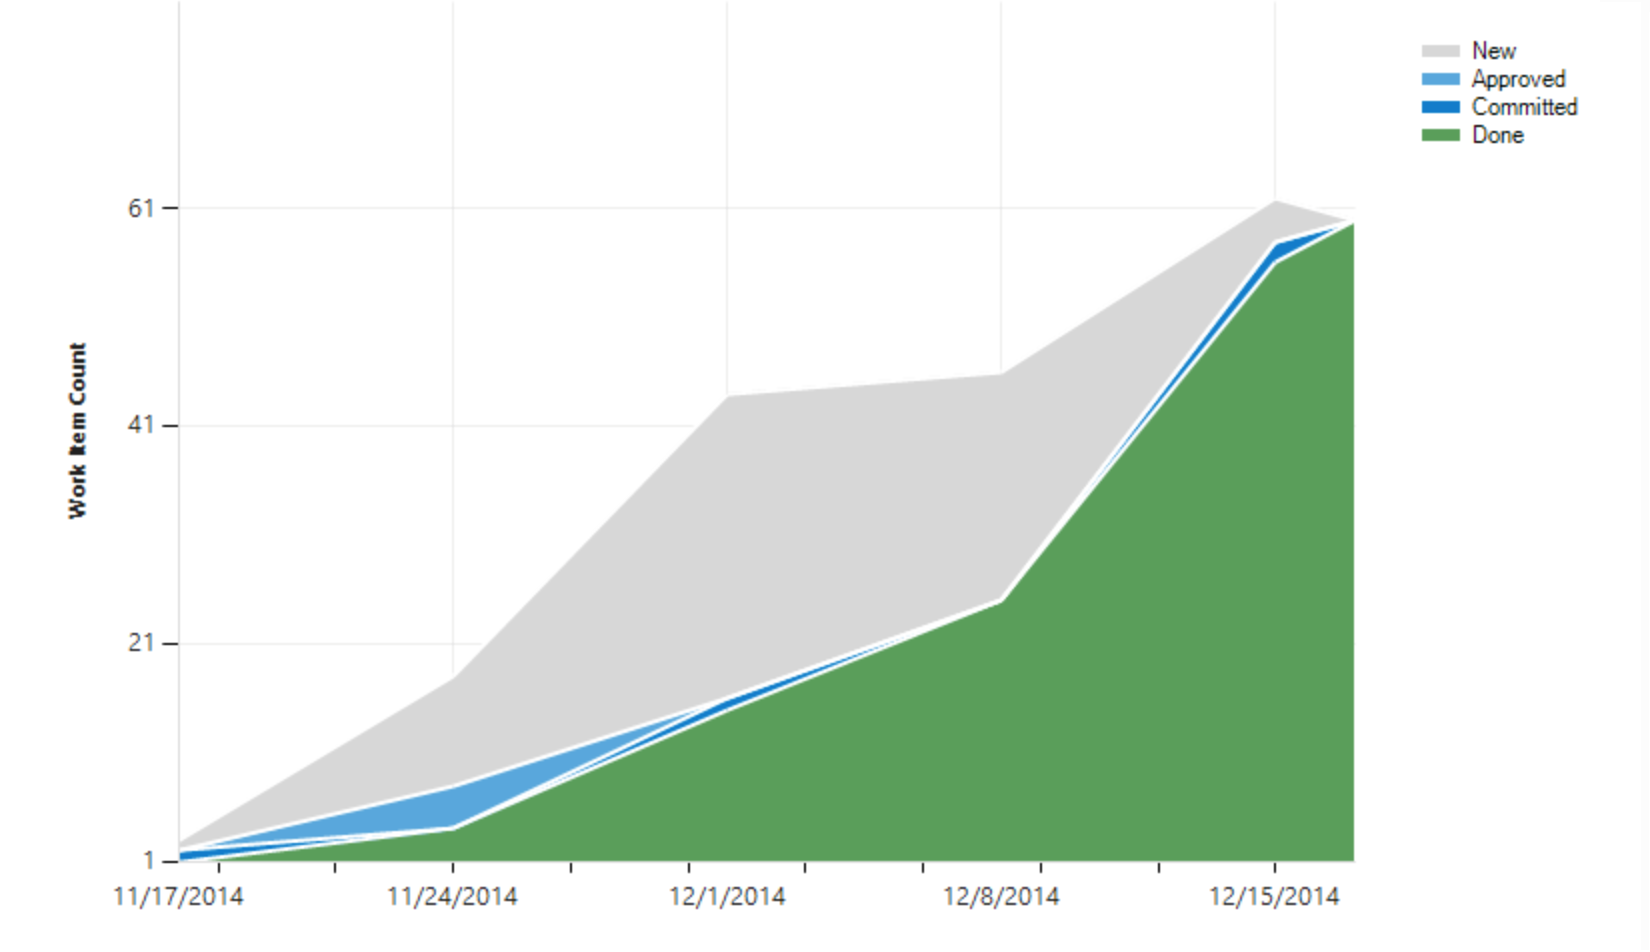
\includegraphics[width=\textwidth]{Figures/TotalGraph}
	\caption{Total work completed graph.}
	\label{fig:totalworkgraph}
\end{figure}
Figure \ref{fig:totalworkgraph} shows the graph of completed work. The graph reflects the fact that more work has been completed later in the time frame of the project. Furthermore it is visible that the use of the tags \textit{Approved} and \textit{Committed} has only been used minimally.\\

The project as an entirety has been a great success, and the \textit{SCRUM} methodology has proven a most valuable tool.